\documentclass[../main.tex]{subfiles}

\begin{document}
\chapter{Fourierreihen}

\begin{motivation}
  Eine Gitarrensaite schwingt mit einer Grundschwingung
  \[
    u_0(x, t) = c_0 \cdot \sin(x) \cdot \cos(t)
  \]
  und Obertönen
  \[
    u_n(x, t) = c_{n+1} \cdot \sin(nx) \cdot \cos(nt),
  \]
  siehe Abbildung~\ref{fig:guitar}.
  Die $u_n$ sind Lösungen der Wellengleichung
  \[
    \frac{\partial^2}{\partial x} u(x, t)
    =
    \frac{\partial^2}{\partial t^2} u(x, t).
  \]
  Das Superpositionsprinzip sagt, dass auch
  $\sum_{k=1}^{n} u_k(x, t)$ eine Lösung
  mit Anfangsprofil 
  \[
    u_0(x, 0) + u_1(x, 0) + \cdots u_n(x, 0)
    = c_0 \sin(x) + c_1 \sin(2x) + \cdots + c_n \sin(nx)
  \]
  ist.
  Wir fragen uns nun, ob wir im Limes $n \to \infty$ 
  jedes Anfangsprofil so ausdrücken können.
  Die physikalische Intuition sagt uns, dass das gehen muss,
  doch es gibt stetige Funktionen auf $[0, \pi]$
  deren Graph unendliche Länge
  hat.
  Hier haben wir keine physikalische Interpretation des
  Anfangsprofils als Gitarrensaite. Die Theorie, die wir hier
  entwickeln, wird jedoch auch für solche Funktionen
  eine positive Antwort liefern.
\end{motivation}

\begin{figure}[htb]
  \centering
  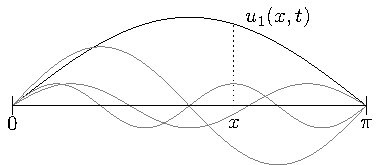
\includegraphics{images/guitar}
  \caption{Eine Gitarrensaite mit weisser Grundschwingung
  und einigen grau eingezeichneten Obertönen}%
  \label{fig:guitar}
\end{figure}


\end{document}
